\section*{\large{DESARROLLO}}
\vspace{-0.25cm}
\justifying

Desarrollo aquí.



\subsubsection*{\it{Sistema de control PID}}
\vspace{-0.25cm}
Para obtener una tensión de salida constante, sin importar variaciones en la tensión de entrada del
convertidor, o en la impedancia de la carga, se implementa un controlador PID.

\begin{figure}[H]
    \centering
    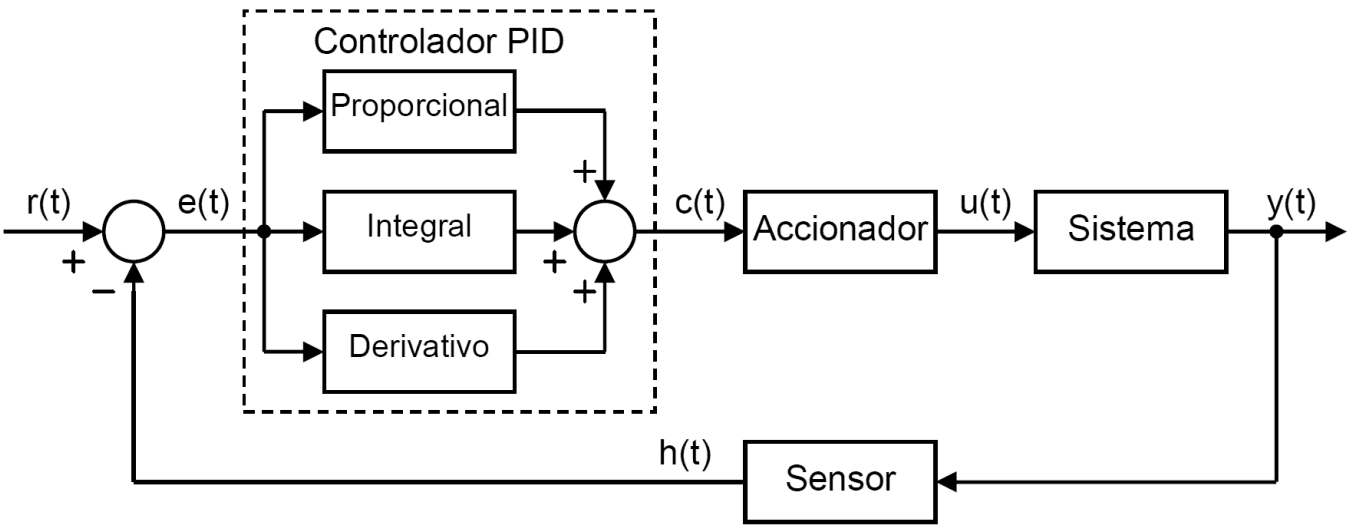
\includegraphics[height=4.5cm]{pid_diagrama.png}
    \vspace{-0.25cm}
    \caption{Diagrama de un sistema de control PID. \parencite{PICUINO}}
    \label{fig:pid_diagrama}
\end{figure}
\vspace{-0.5cm}

Donde:
\begin{itemize}[noitemsep]
    \item $r(t)$ es la señal de referencia, que indica el valor deseado a la salida del sistema.
    \item $h(t)$ es la señal de retroalimentación, que es la medición de un sensor de la salida del sistema.
    \item $e(t)$ es la señal de error, que es la diferencia entre la señal de referencia y la señal de
          retroalimentación del sistema.
    \item $c(t)$ es la señal de control, que es la salida del controlador PID.
    \item $u(t)$ es la señal de entrada al sistema.
    \item $y(t)$ es la salida del sistema.
\end{itemize}

El controlador PID consiste de tres acciones de control diferentes, que se suman para poder
obtener la señal de control. Estas acciones son:

\textbf{Acción de control proporcional (P):} es simplemente la multiplicación de la señal de error por
una constante $K_p$. Esto significa que su acción es proporcional al error. Su función de transferencia es:

\vspace{-0.5cm}
\begin{equation}
    \dfrac{U(s)}{E(s)} = K_p
\end{equation}
\vspace{-0.5cm}

\textbf{Acción de control integral (I):} es la suma acumulada de la señal de error en el tiempo, multiplicada
por una constante $K_i$. Su función de transferencia es:

\vspace{-0.5cm}
\begin{equation}
    \dfrac{U(s)}{E(s)} = \dfrac{K_i}{s}
\end{equation}
\vspace{-0.5cm}

\textbf{Acción de control derivativa (D):} es la derivada de la señal de error en el tiempo, multiplicada por
una constante $K_d$. Su función de transferencia es:

\vspace{-0.5cm}
\begin{equation}
    \dfrac{U(s)}{E(s)} = K_d \cdot s
\end{equation}
\vspace{-0.5cm}

Para reducir el ruido de alta frecuencia en la señal de control, así como para evitar inestabilidades
en el sistema, se utiliza un filtro pasa-bajos en la acción derivativa. La función de transferencia es:

\vspace{-0.5cm}
\begin{equation}
    \dfrac{U(s)}{E(s)} = K_d \cdot \dfrac{N}{1+\dfrac{N}{s}}
\end{equation}
\vspace{-0.5cm}

Sumando las tres acciones de control, obtenemos la función de transferencia en forma paralela del controlador PID:

\vspace{-0.5cm}
\begin{equation}
    \dfrac{U(s)}{E(s)} = K_p + \dfrac{K_i}{s} + K_d \cdot \dfrac{N}{1+\dfrac{N}{s}}
\end{equation}
\vspace{-0.5cm}

Como en nuestro sistema de control se utiliza un microcontrolador, se debe discretizar la función de transferencia
del controlador PID para implementarla correctamente. Utilizando la transformación de Euler, se obtiene la siguiente
función de transferencia discreta:

\vspace{-0.5cm}
\begin{equation}
    \dfrac{U(s)}{E(s)} = K_p + K_i \cdot \dfrac{T_s}{z-1} + K_d \cdot \dfrac{N}{1+N \cdot \dfrac{T_s}{z-1}}
\end{equation}
\vspace{-0.5cm}

Aplicando denominador común y agrupando términos, se obtiene:

\vspace{-0.5cm}
\begin{equation}
    \dfrac{U(z)}{E(z)} =
    \frac
    {
        \splitfrac{
            (K_p + K_d N)\ z^2 + (-2 K_p - 2 K_d N + K_i T_s + K_p N T_s)\ z
        }{
            + (K_p + K_d N - K_i T_s - K_p N T_s + K_i N {T_s}^2)
        }
    }
    {
            z^2 + (-2 + N T_s) z + (1 - N T_s)
    }
    \end{equation}
\vspace{-0.5cm}

Finalmente, se puede obtener la ecuación en diferencias del controlador PID:

\vspace{-0.5cm}
\begin{multline}
        u[n] = (K_p + K_d N)\ e[n] + (-2 K_p - 2 K_d N + K_i T_s + K_p N T_s)\ e[n-1]\  + \\
    (K_p + K_d N - K_i T_s - K_p N T_s + K_i N {T_s}^2)\ e[n-2] - (2 - N T_s)\ u[n-1] - (1 - N T_s)\ u[n-2]
\end{multline}
\vspace{-0.5cm}

\subsubsection*{\it{Modelado del sistema}}
\vspace{-0.25cm}
Primero, la fuente se incluye en el circuito cuando el interruptor esta conectado al nodo 1.
El convertidor Buck se puede modelar de la siguiente manera.

\vspace{-0.5cm}
\begin{equation}
    \begin{bmatrix}
        i_U\\
        i_C\\
        i_{R_C}\\
        i_{R_L}\\
        u_L\\
        u_I\\
    \end{bmatrix}
    =
    \begin{bmatrix}
        0 & 0 & 0 & 0 & 1 & 0\\
        0 & 0 & 0 & 0 & 1 & -1\\
        0 & 0 & 0 & 0 & 1 & -1\\
        0 & 0 & 0 & 0 & 1 & 0\\
        -1 & -1 & -1 & -1 & 0 & 0\\
        0 & 1 & 1 & 0 & 0 & 0\\
    \end{bmatrix}
    \cdot
    \begin{bmatrix}
        u_U\\
        u_C\\
        u_{R_C}\\
        u_{R_L}\\
        i_L\\
        i_I\\
    \end{bmatrix}
\end{equation}

Donde u es el voltage del convertidor e i es la corriente.
Modelando los dos componentes de almacenamiento de energía que tiene:

\vspace{-0.5cm}
\begin{equation}
    \begin{bmatrix}
        i_C \\
        u_L
    \end{bmatrix}
    =
    \begin{bmatrix}
        0 & 1 \\
        -1 & 0
    \end{bmatrix}
    \cdot
    \begin{bmatrix}
        u_C \\
        i_L
    \end{bmatrix}
    +
    \begin{bmatrix}
        0 & -1 \\
        -1 & 0
    \end{bmatrix}
    \cdot
    \begin{bmatrix}
        u_U \\
        i_I
    \end{bmatrix}
    +
    \begin{bmatrix}
        0 & 0 \\
        -1 & -1
    \end{bmatrix}
    \cdot
    \begin{bmatrix}
        u_{R_C} \\
        u_{R_L}
    \end{bmatrix}
\end{equation}

Dado que el voltaje de salida es la suma del voltaje del capacitor y del voltaje del resistor, 
donde el voltaje del resistor es el producto de la corriente y la resistencia, entonces se tiene que:

\vspace{-0.75cm}
\begin{equation}
    u_0 = u_C + u_{R_C}
\end{equation}
\vspace{-0.75cm}

\vspace{-0.75cm}
\begin{equation}
    u_{R_C} = R_C \cdot i_L
\end{equation}
\vspace{-0.75cm}


\begin{equation}
    u_0 = u_C + u_{R_C} = [1 \ \ R_C] 
    \begin{bmatrix}
        u_C \\
        i_L
    \end{bmatrix}
\end{equation}
\vspace{-0.5cm}



\begin{equation}
    \begin{bmatrix}
        i_C \\
        u_L
    \end{bmatrix}
    =
    \begin{bmatrix}
        0 & 1 \\
        -1 & -R_C - R_L
    \end{bmatrix}
    \cdot
    \begin{bmatrix}
        u_C \\
        i_L
    \end{bmatrix}
    +
    \begin{bmatrix}
        0 \\
        -1
    \end{bmatrix}
\end{equation}


\begin{equation}
        u_0 = [1 \ \ R_C] 
    \begin{bmatrix}
        u_C \\
        i_L
    \end{bmatrix}
\end{equation}

Incluyendo las ecuaciones constitutivas, el sistema se modela como:

\begin{equation}
    \begin{bmatrix}
        \dfrac{d}{dt}u_C\\
        \dfrac{d}{dt}i_L
    \end{bmatrix}
    =
    \begin{bmatrix}
        0 & \dfrac{1}{C}\\
        -\dfrac{1}{L} & -\dfrac{R_C + R_L}{L}
    \end{bmatrix}
    \cdot
    \begin{bmatrix}
        u_C\\
        i_L
    \end{bmatrix}
    +
    \begin{bmatrix}
        0 & -\dfrac{1}{C}\\
        -\dfrac{1}{L} & -\dfrac{R_C}{L}
    \end{bmatrix}
    \cdot
    \begin{bmatrix}
        u_U\\
        i_I
    \end{bmatrix}  
\end{equation}

\begin{equation}
    \begin{bmatrix}
        u_0\\
        i_L
    \end{bmatrix}
    =
    \begin{bmatrix}
        1 & R_C\\
        0 & 1
    \end{bmatrix}
    \begin{bmatrix}
        u_C\\
        i_L
    \end{bmatrix}
    +
    \begin{bmatrix}
        0 & 0\\
        0 & 0
    \end{bmatrix}
    \cdot
    \begin{bmatrix}
        u_U\\
        i_I
    \end{bmatrix}
\end{equation}

El sistema de ecuaciones en espacio de estado esta dado por:

\begin{equation}
    \begin{cases}
    \dot{x} = Ax + Bu \\
    y = Cx
    \end{cases}
\end{equation}

Donde u es la entrada del sistema e y la salida.
Cuando el interruptor esta conectado al nodo dos, las fuente de tension 
no se incluye en el circuito.

\begin{equation}
    \begin{bmatrix}
        i_C\\
        i_{R_C}\\
        i_{R_L}\\
        u_L\\
        u_I\\
    \end{bmatrix}
    =
    \begin{bmatrix}
        0 & 0 & 0 & 1 & -1\\
        0 & 0 & 0 & 1 & -1\\
        0 & 0 & 0 & 1 & -1\\
        -1 & -1 & -1 & 0 & 0\\
        1 & 1 & 0 & 0 & 0\\
    \end{bmatrix}
    \cdot
    \begin{bmatrix}
        u_C\\
        u_{R_C}\\
        u_{R_L}\\
        i_L\\
        i_I\\
    \end{bmatrix}
\end{equation}

Modelando los dos componentes de almacenamiento de energía que tiene:

\begin{equation}
    \begin{bmatrix}
        i_C \\
        u_L
    \end{bmatrix}
    =
    \begin{bmatrix}
        0 & 1 \\
        -1 & 0
    \end{bmatrix}
    \cdot
    \begin{bmatrix}
        u_C \\
        i_L
    \end{bmatrix}
    +
    \begin{bmatrix}
        0 & 0 \\
        -1 & -1
    \end{bmatrix}
    \cdot
    \begin{bmatrix}
        u_{R_C} \\
        u_{R_L}
    \end{bmatrix}
    +
    \begin{bmatrix}
        -1 \\
        0
    \end{bmatrix}
    \cdot
    i_I
\end{equation}

Incluyendo las ecuaciones constitutivas, el sistema se modela como:

\begin{equation}
    \begin{bmatrix}
        \dfrac{d}{dt}u_C\\
        \dfrac{d}{dt}i_L
    \end{bmatrix}
    =
    \begin{bmatrix}
        0 & \dfrac{1}{C}\\
        -\dfrac{1}{L} & -\dfrac{R_C + R_L}{L}
    \end{bmatrix}
    \cdot
    \begin{bmatrix}
        u_C\\
        i_L
    \end{bmatrix}
    +
    \begin{bmatrix}
        -\dfrac{1}{C}\\
        -\dfrac{R_C}{L}
    \end{bmatrix}
    \cdot
   i_I 
\end{equation}

El sistema de ecuaciones en sistema de estado viene dado por:

\begin{equation}
    \begin{bmatrix}
        \dfrac{d}{dt}u_C\\
        \dfrac{d}{dt}i_L
    \end{bmatrix}
    =
    \begin{bmatrix}
        0 & \dfrac{1}{C}\\
        -\dfrac{1}{L} & -\dfrac{R_C + R_L}{L}
    \end{bmatrix}
    \cdot
    \begin{bmatrix}
        u_C\\
        i_L
    \end{bmatrix}
    +
    \begin{bmatrix}
        0 & -\dfrac{1}{C}\\
        0 & -\dfrac{R_C}{L}
    \end{bmatrix}
    \cdot
    \begin{bmatrix}
        u_U\\
        i_I
    \end{bmatrix} 
\end{equation}

\begin{equation}
    \begin{bmatrix}
        u_0\\
        i_L
    \end{bmatrix}
    =
    \begin{bmatrix}
        1 & R_C\\
        0 & 1
    \end{bmatrix}
    \begin{bmatrix}
        u_C\\
        i_L
    \end{bmatrix}
\end{equation}

OBTENER SISTEMA PROMEDIO

El sistema promediado en el tiempo se puede derivar como la ponderación promediada de
los dos sistemas. Sistema S1 con fuente de voltaje y sistema S2
sin fuente de voltaje. Suponiendo el ciclo de trabajo d, tenemos:

\begin{equation}
    S_{Promedio} = d \cdot S_1 + (1 - d) \cdot S_2
\end{equation}

Como se puede observar en las matrices ABCD de los dos sistemas, las matrices ACD
son iguales mientras que la matriz B es diferente.
Entonces solo es necesario tomar el valor promedio de la matriz B.

\begin{equation}
    B_{Promedio} = d \cdot B_1 + (1 - d) \cdot B_2
\end{equation}

La matriz B se puede escribir como:

\begin{equation}
    B_{Promedio} = d \cdot (B_11 + B_12) + (1 - d) \cdot (B_21 + B_22)
\end{equation}

\[
\text{Donde: } B_{11} = \begin{bmatrix}
0 & 0 \\
\frac{1}{L} & 0
\end{bmatrix}
\quad \text{y} \quad
B_{12} = \begin{pmatrix}
0 & -\frac{1}{C_c} \\
0 & \frac{R_c}{L}
\end{pmatrix}
\]

\[
B_{21} = \begin{bmatrix}
0 & 0 \\
0 & 0
\end{bmatrix}
\quad \text{y} \quad
B_{22} = \begin{bmatrix}
0 & -\frac{1}{C_c} \\
0 & \frac{R_c}{L}
\end{bmatrix}
\]

Escribiendo el sistema en tiempo continuo:

\begin{equation}
    \begin{bmatrix}
        \dfrac{d}{dt}u_C\\
        \dfrac{d}{dt}i_L
    \end{bmatrix}
    =
    \begin{bmatrix}
        0 & \dfrac{1}{C}\\
        -\dfrac{1}{L} & -\dfrac{R_C + R_L}{L}
    \end{bmatrix}
    \cdot
    \begin{bmatrix}
        u_C\\
        i_L
    \end{bmatrix}
    +
    \begin{bmatrix}
        0 & -\dfrac{I_0}{C_C}\\
        -\dfrac{V_g}{L} & -\dfrac{R_C}{L}
    \end{bmatrix}
    \cdot
    \begin{bmatrix}
        d\\
        I_0
    \end{bmatrix} 
\end{equation}

Dado que B es el resultado promediado del sistema conmutado y los valores del voltaje de entrada,
el capacitor, la resistencia y el inductor son fijos, entonces B será decidido por el ciclo de
trabajo $d$. El valor de B cambiará cuando cambie el ciclo de trabajo $d$.



\subsubsection*{\it{Identificación del sistema}}
\vspace{-0.25cm}
Si bien el modelo del sistema se puede obtener a partir de las ecuaciones de Kirchhoff, se procede
a obtener un modelo empírico. Para ello, se aplica una señal de entrada al sistema físico y se
mide la respuesta del mismo.

En esta ocasión, se optó por utilizar una señal de entrada PRBS
(Pseudo Random Binary Sequence, en español Secuencia Binaria Pseudo Aleatoria). La misma intenta
cubrir todo el rango de frecuencias posibles, y es útil para identificar sistemas lineales y no lineales.
Utilizando MATLAB, se genera una señal PRBS de orden 10, con un tiempo de muestreo de 200 microsegundos,
y una duración de 3 períodos. Esto significa una secuencia de 1023 valores en 0,2046 segundos repetida tres veces.
Es decir, 3069 valores en un rango de 0 a 0,6138 segundos.

Se programa el microcontrolador para reproducir la señal PRBS en el convertidor Buck, medir la salida
del sistema y luego enviar los datos mediante comunicación serial. A través de un programa en Python, se guardan
los valores en un archivo csv para luego introducir en el System Identification Toolbox de MATLAB:


\begin{figure}[H]
    \centering

    \begin{subfigure}[b]{\textwidth}
        \centering
        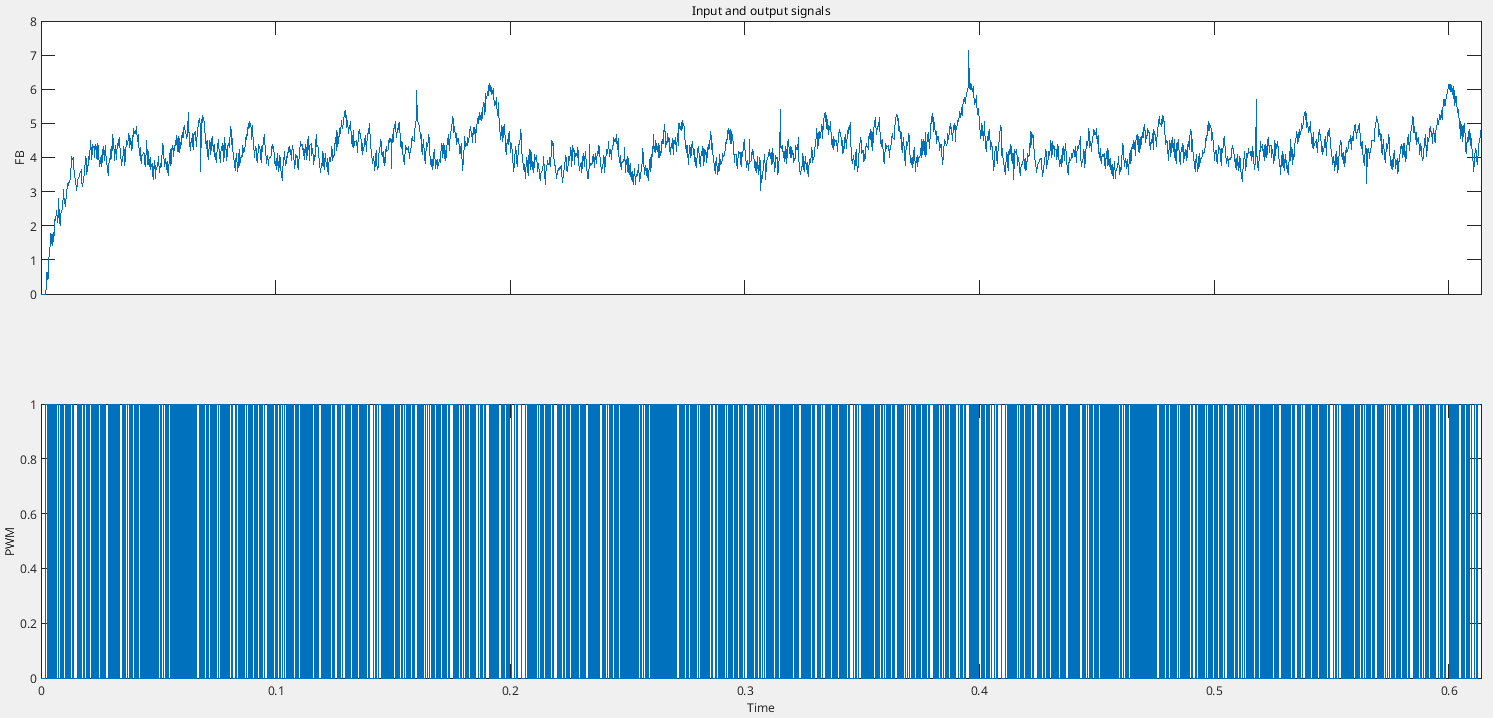
\includegraphics[height=6cm]{identificacion_io.png}
        %\vspace{-0.25cm}
        \caption{Vista completa de la señal de identificación.}
        \label{fig:identificacion_io_gral}
    \end{subfigure}
    \begin{subfigure}[b]{\textwidth}
        \centering
        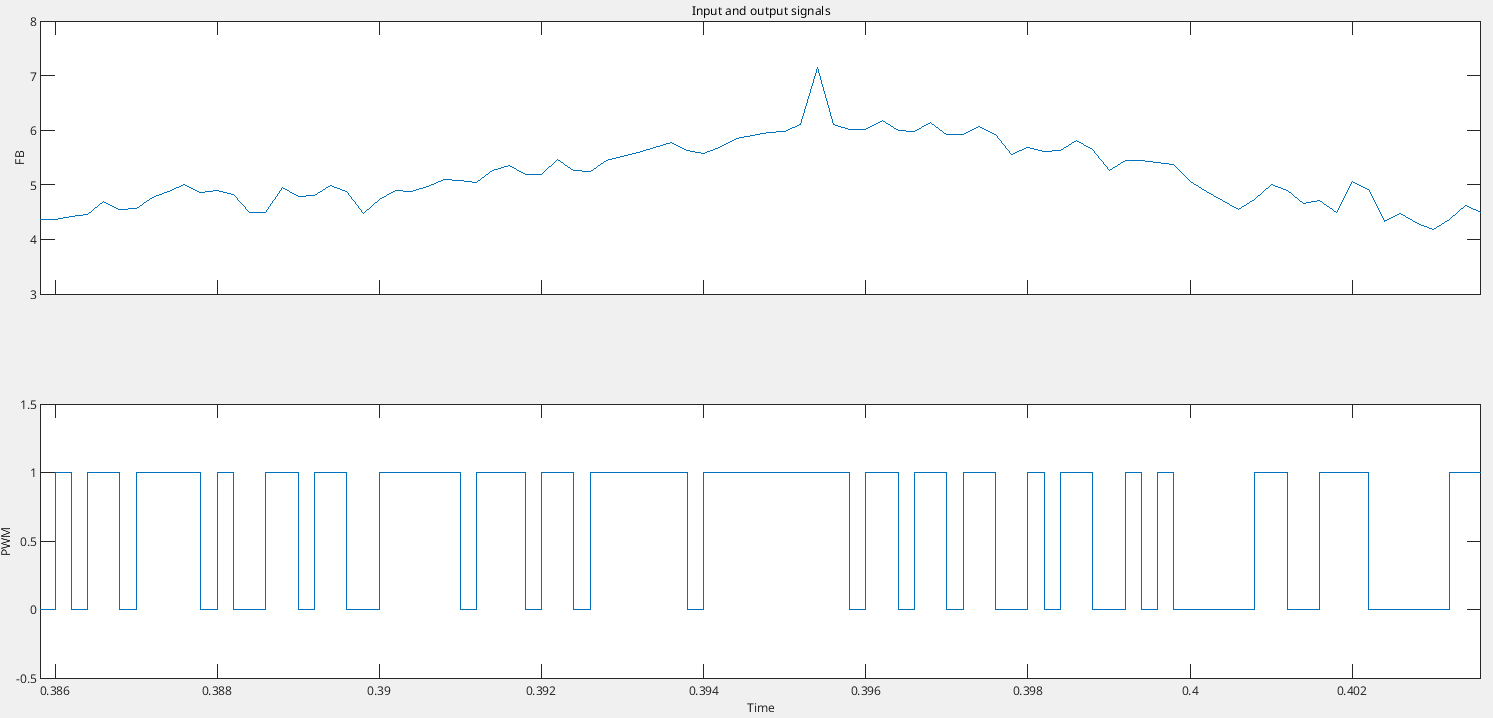
\includegraphics[height=6cm]{identificacion_zoom.png}
        %\vspace{-0.25cm}
        \caption{Vista acercada de la señal de identificación.}
        \label{fig:identificacion_io_zoom}
    \end{subfigure}

    \vspace{-0.25cm}
    \caption{Salida (arriba) y entrada (abajo) del sistema con la señal de identificación.}
    \label{fig:identificacion_io}
\end{figure}
\vspace{-0.5cm}

Se seleccionan los primeros 2455 valores (80\% de los valores totales) como la señal de evaluación
y los restantes 614 valores (20\% de los valores totales) como la señal de validación. Finalmente,
se estima un modelo en espacios de estado de orden 2 utilizando la función \textit{N4SID} del System Identification Toolbox:

\begin{figure}[H]
    \centering

    \begin{subfigure}[b]{\textwidth}
        \centering
        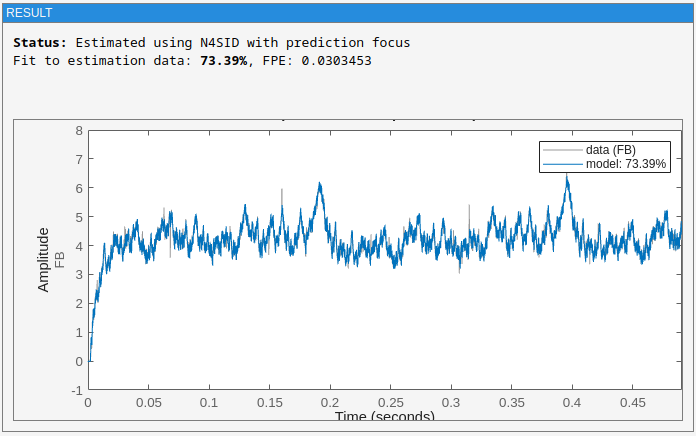
\includegraphics[width=10cm]{identificacion_comparacion.png}
        %\vspace{-0.25cm}
        \caption{Comparación del modelo estimado con la respuesta medida.}
        \vspace{0.25cm}
        \label{fig:identificacion_comparacio n}
    \end{subfigure}
    \begin{subfigure}[b]{\textwidth}
        \centering
        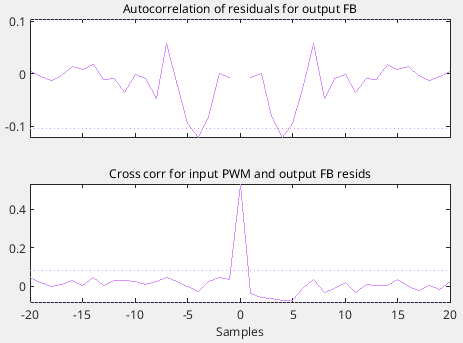
\includegraphics[width=10cm]{identificacion_residuos.png}
        %\vspace{-0.25cm}
        \caption{Análisis residual del modelo estimado.}
        \label{fig:identificacion_residuos}
    \end{subfigure}

    \vspace{-0.25cm}
    \caption{Resultados de la estimación del modelo del sistema.}
    \label{fig:identificacion_resultados}
\end{figure}
\vspace{-0.5cm}

Como se puede observar en la Figura \ref{fig:identificacion_resultados}, el modelo estimado coincide
con la respuesta medida del sistema (señal de evaluación) en un 73,39\%. Respecto a la señal de 
validación, coincide en un 65,8\%. Además, el análisis residual del modelo estimado
demuestra un buen resultado en la autocorrelación de residuales para la salida y un resultado
satisfactorio para la correlación cruzada de residuales entre la entrada y la salida.

El modelo estimado en espacios de estado es el siguiente:

\vspace{-0.5cm}
\begin{equation}
    \begin{cases}
        \begin{bmatrix}
            \dot{x_1}\\
            \dot{x_2}
        \end{bmatrix}
        =
        \begin{bmatrix}
            -213.1  &   279.1\\
            2819    &   -1.178\times 10^4
        \end{bmatrix}
        \cdot
        \begin{bmatrix}
            x_1 \\
            x_2
        \end{bmatrix}
        +
        \begin{bmatrix}
            -28.98 \\
            294,4
        \end{bmatrix}
        \cdot
        u 
        +
        \begin{bmatrix}
            -11.92 \\
            -95.37
        \end{bmatrix}
        \cdot
        e
        \\
        y =
        \begin{bmatrix}
            -56.54 & 4.834
        \end{bmatrix}
        \cdot
        \begin{bmatrix}
            x_1 \\
            x_2
        \end{bmatrix}
        +
        e

    \end{cases}
\end{equation}

El mismo se puede representar en función de transferencia luego de transformarlo mediante MATLAB:

\vspace{-0.5cm}
\begin{equation}
    H(s) = \dfrac{3062\ s + 1.456 \times 10^7}{s^2 + 1.199 \times 10^4\ s + 1.722 \times 10^6}
\end{equation}
\vspace{-0.5cm}

La planta discretizada mediante retención de orden cero (zoh), con un tiempo de muestreo de 200
microsegundos es:

\vspace{-0.5cm}
\begin{equation}
    H(z) = \dfrac{0.3798\ z - 0.1602}{z^2 - 1.065\ z + 0.09091}
\end{equation}
\vspace{-0.5cm}

\begin{figure}[H]
    \centering

    \begin{subfigure}[b]{0.49\textwidth}
        \centering
        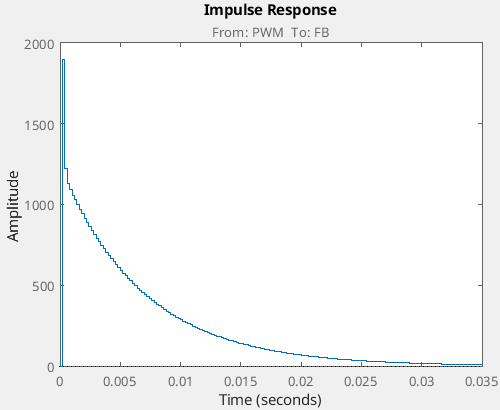
\includegraphics[width=\textwidth]{estimado_impulse.png}
        %\vspace{-0.25cm}
        \caption{Respuesta al impulso.}
        \label{fig:estimado_impulse}
    \end{subfigure}
    \begin{subfigure}[b]{0.49\textwidth}
        \centering
        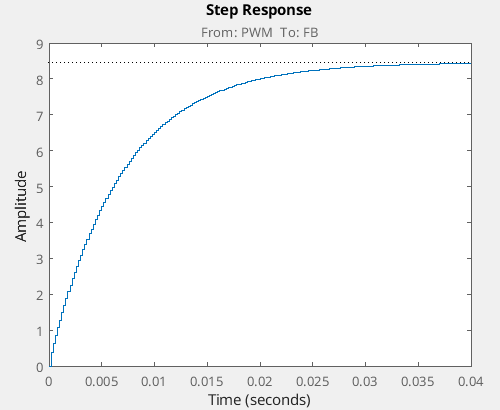
\includegraphics[width=\textwidth]{estimado_step.png}
        %\vspace{-0.25cm}
        \caption{Respuesta al escalón.}
        \label{fig:estimado_step}
    \end{subfigure}

    \vspace{-0.25cm}
    \caption{Análisis de la respuesta temporal del sistema estimado.}
    \label{fig:estimado_respuestas}
\end{figure}
\vspace{-0.5cm}

\begin{figure}[H]
    \centering

    \begin{subfigure}[b]{0.49\textwidth}
        \centering
        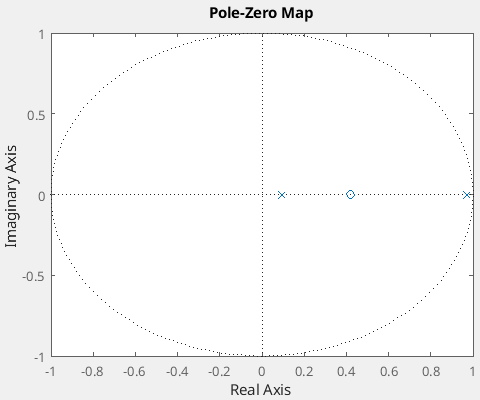
\includegraphics[width=\textwidth]{estimado_pzmap.png}
        %\vspace{-0.25cm}
        \caption{Mapa de polos y ceros.}
        \label{fig:estimado_pzmap}
    \end{subfigure}
    \begin{subfigure}[b]{0.49\textwidth}
        \centering
        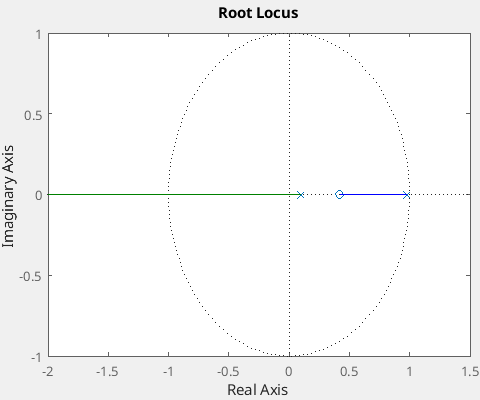
\includegraphics[width=\textwidth]{estimado_rlocus.png}
        %\vspace{-0.25cm}
        \caption{Lugar geométrico de las raíces.}
        \label{fig:estimado_rlocus}
    \end{subfigure}

    \vspace{-0.25cm}
    \caption{Análisis de la respuesta temporal del sistema estimado.}
    \label{fig:estimado_estabilidad}
\end{figure}
\vspace{-0.5cm}
